%<dscrpt>Période 3 implique chaos.</dscrpt>
Ce problème illustre la complexité du comportement des suites définies par récurrence dans le cas où la fonction n'est pas monotone. Il introduit à un résultat connu comme
\begin{center}
  \og Période 3 implique chaos. \fg
\end{center}

\begin{figure}[h]
  \centering
  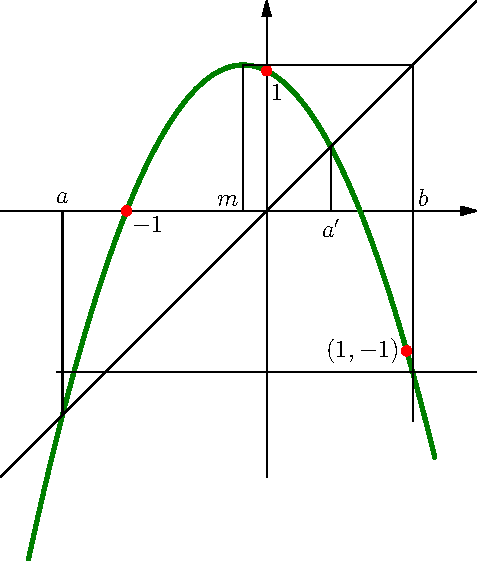
\includegraphics{./Ep3impko_1.pdf}
  % Ep3impko_1.pdf: 0x0 pixel, -2147483648dpi, 0.00x0.00 cm, bb=
  \caption{Graphe de $f$}
  \label{fig: Ep3impko_1}
\end{figure}

\subsection*{Partie I. La fonction.}
\begin{enumerate}
  \item Déterminer les réels $a$, $b$, $c$ tels que la fonction polynomiale $f$ définie par 
\begin{displaymath}
  \forall x\in\R,\; f(x) = ax^2 + bx + c
\end{displaymath}
vérifie $f(-1) = 0$, $f(0) = 1$, $f(1) = -1$.

  \item Justifier avec un tableau de variations que le graphe présenté en figure \ref{fig: Ep3impko_1} est celui de $f$. Préciser les valeurs de $a$, $m$, $a'$, $b$. On ne demande pas de vérifier les inégalités suivantes visibles sur le graphe mais on pourra les utiliser dans la suite.
\begin{displaymath}
f(x) - x 
\left\lbrace 
\begin{aligned}
  < 0 &\text{ si } x \notin \left[ a, a' \right]  \\
  > 0 &\text{ si } x \in \left] a, a' \right[
\end{aligned}
\right., \hspace{1cm}
a < f(b) < -1 < m < 0 < a' < 1 < b
\end{displaymath}

  \item Avec des éléments de la chaîne d'inégalités du dessus, exprimer
\begin{displaymath}
  f(\left] -\infty , a\right]),\hspace{0.5cm} f([a,m]),\hspace{0.5cm} f([m,b]).
\end{displaymath}
En déduire $f([a,b])\subset [a,b]$.

  \item On définit une suite $\left( x_n\right)_{n\in \N}$ par :
  \begin{displaymath}
x_0 \in \R, \hspace{0.5cm} \forall n\in \N, \; x_{n+1} = f(x_n)    
  \end{displaymath}
\'Etudier cette suite dans les cas suivants
\begin{displaymath}
  x_0 < a, \hspace{0.5cm} x_0 = a, \hspace{0.5cm} x_0 = -1, \hspace{0.5cm} x_0 = 0, \hspace{0.5cm}
   x_0 = a', \hspace{0.5cm} x_0 = 1.
\end{displaymath}
\end{enumerate}

\subsection*{Partie II. Les outils.}  
\begin{enumerate}
  \item Pour $u < v$ réels, soit $J=\left[ u, v \right]$ et $g \in \mathcal{C}(J,\R)$ telle que $J \subset g(J)$. 
  Montrer que $g$ admet un point fixe dans $J$ c'est à dire qu'il existe $x\in J$ tel que $g(x) = x$  (on pourra considérer $z$ et $t$ dans $J$ tels que $g(z)=u$ et $g(t)=v$).
  
  \item Soit $I$ un segment de $\R$, $f \in \mathcal{C}(I,\R)$ et $K=\left[ v,V\right] \subset f(I)$ avec $v < V$. 
  On veut montrer qu'il existe $\alpha$ et $\beta$ dans $I$ tels que $K=f(\left[ \alpha, \beta\right])$.\newline
  Comme $\left[ v,V\right]\subset f(I)$, il existe $a$ et $b$ dans $I$ tels que $v=f(a)$ et $V=f(b)$. On suppose $a < b$ dans les questions a., b., c..
\begin{enumerate}
  \item Soit $A = \left\lbrace x\in \left[a,b\right] \text{ tq } f(x) = v \right\rbrace$. Montrer que $A$ admet un plus grand élément (noté $\alpha$). Montrer que $\alpha < b$ et que
  \begin{displaymath}
    \alpha < x \leq b \Rightarrow v < f(x)
  \end{displaymath}
  \item Soit $B = \left\lbrace x\in \left[\alpha,b\right] \text{ tq } f(x) = V \right\rbrace$. Montrer que $B$ admet un plus petit élément (noté $\beta$). Montrer que $\alpha < \beta$ et que
  \begin{displaymath}
    \alpha \leq x < \beta \Rightarrow  f(x) < V
  \end{displaymath}
  \item Montrer que $[v,V] = f(\left[\alpha, \beta \right])$. 
  \item Comment faire dans le cas $b<a$?
\end{enumerate}
\end{enumerate}

\subsection*{Partie III. Existence de suites périodiques.}
On se replace dans le contexte de la première partie en notant $I_-=\left[ -1,0\right]$ et $I_+=\left[ 0 , 1\right]$.\newline
On veut montrer qu'il existe un $c\in I_+$ tel que 
\begin{displaymath}
  f\circ f \circ f \circ f(c) = c \text{ avec } f(c)\neq c, \; f\circ f (c) \neq c,\; f\circ f \circ f (c) \neq c 
\end{displaymath}
On pourra noter $f^i = \underset{i \text{ fois }}{\underbrace{f\circ f \circ \cdots \circ f}}$.
\begin{enumerate}
  \item Préciser $f(I_-)$ et $f(I_+)$ avec $a$, $f(b)$, $m$, $a'$ et $b$. En déduire
\begin{displaymath}
  I_+ \subset f(I_-),\hspace{0.5cm} I_- \subset f(I_+),\hspace{0.5cm} I_+ \subset f(I_+)
\end{displaymath}
  \item 
\begin{enumerate}
  \item Montrer qu'il existe des segments $K_1$, $K_2$, $K_3$, $K_4$ tels que 
\begin{multline*}
  \left( K_1 \subset I_+ \text{ et } f(K_1)= I_+\right), \hspace{0.5cm} 
  \left( K_2 \subset K_1 \subset I_+ \text{ et } f(K_2)= K_1\right), \hspace{0.5cm}\\
  \left( K_3 \subset I_- \text{ et } f(K_3)= K_2\right), \hspace{0.5cm}
  \left( K_4 \subset I_+ \text{ et } f(K_4)= K_3\right)
\end{multline*}
  \item Reproduire sur votre copie la figure \ref{fig: Ep3impko_1} et présenter les segments $K_1$, $K_2$, $K_3$, $K_4$ estimés graphiquement.
\end{enumerate}

  \item Montrer qu'il existe $c\in K_4$ tel que $f^4(c) = c$.
  
  \item Pour le $c$ défini dans la question précédente, montrer que
\begin{displaymath}
\left( c=f(c) \Rightarrow c=0\right),\hspace{0.5cm} \left( c =f\circ f(c) \Rightarrow f(c)=0\right),\hspace{0.5cm}
\left( c=f^3(c) \Rightarrow c=0\right)
\end{displaymath}
Conclure.

  \item Montrer qu'il existe $c_2\in I_+$ tel que $f(c_2)\neq c_2$ et $f\circ f(c_2) = c_2$.
  
  \item Montrer que, pour tout entier $n\geq 3$, il existe $c_n\in I_+$ tel que la suite définie par récurrence avec la condition initiale $c_n$ soit périodique de plus petite période $n$.  
\end{enumerate}
